% GNUPLOT: LaTeX picture with Postscript
\begingroup
  \makeatletter
  \providecommand\color[2][]{%
    \GenericError{(gnuplot) \space\space\space\@spaces}{%
      Package color not loaded in conjunction with
      terminal option `colourtext'%
    }{See the gnuplot documentation for explanation.%
    }{Either use 'blacktext' in gnuplot or load the package
      color.sty in LaTeX.}%
    \renewcommand\color[2][]{}%
  }%
  \providecommand\includegraphics[2][]{%
    \GenericError{(gnuplot) \space\space\space\@spaces}{%
      Package graphicx or graphics not loaded%
    }{See the gnuplot documentation for explanation.%
    }{The gnuplot epslatex terminal needs graphicx.sty or graphics.sty.}%
    \renewcommand\includegraphics[2][]{}%
  }%
  \providecommand\rotatebox[2]{#2}%
  \@ifundefined{ifGPcolor}{%
    \newif\ifGPcolor
    \GPcolortrue
  }{}%
  \@ifundefined{ifGPblacktext}{%
    \newif\ifGPblacktext
    \GPblacktexttrue
  }{}%
  % define a \g@addto@macro without @ in the name:
  \let\gplgaddtomacro\g@addto@macro
  % define empty templates for all commands taking text:
  \gdef\gplbacktext{}%
  \gdef\gplfronttext{}%
  \makeatother
  \ifGPblacktext
    % no textcolor at all
    \def\colorrgb#1{}%
    \def\colorgray#1{}%
  \else
    % gray or color?
    \ifGPcolor
      \def\colorrgb#1{\color[rgb]{#1}}%
      \def\colorgray#1{\color[gray]{#1}}%
      \expandafter\def\csname LTw\endcsname{\color{white}}%
      \expandafter\def\csname LTb\endcsname{\color{black}}%
      \expandafter\def\csname LTa\endcsname{\color{black}}%
      \expandafter\def\csname LT0\endcsname{\color[rgb]{1,0,0}}%
      \expandafter\def\csname LT1\endcsname{\color[rgb]{0,1,0}}%
      \expandafter\def\csname LT2\endcsname{\color[rgb]{0,0,1}}%
      \expandafter\def\csname LT3\endcsname{\color[rgb]{1,0,1}}%
      \expandafter\def\csname LT4\endcsname{\color[rgb]{0,1,1}}%
      \expandafter\def\csname LT5\endcsname{\color[rgb]{1,1,0}}%
      \expandafter\def\csname LT6\endcsname{\color[rgb]{0,0,0}}%
      \expandafter\def\csname LT7\endcsname{\color[rgb]{1,0.3,0}}%
      \expandafter\def\csname LT8\endcsname{\color[rgb]{0.5,0.5,0.5}}%
    \else
      % gray
      \def\colorrgb#1{\color{black}}%
      \def\colorgray#1{\color[gray]{#1}}%
      \expandafter\def\csname LTw\endcsname{\color{white}}%
      \expandafter\def\csname LTb\endcsname{\color{black}}%
      \expandafter\def\csname LTa\endcsname{\color{black}}%
      \expandafter\def\csname LT0\endcsname{\color{black}}%
      \expandafter\def\csname LT1\endcsname{\color{black}}%
      \expandafter\def\csname LT2\endcsname{\color{black}}%
      \expandafter\def\csname LT3\endcsname{\color{black}}%
      \expandafter\def\csname LT4\endcsname{\color{black}}%
      \expandafter\def\csname LT5\endcsname{\color{black}}%
      \expandafter\def\csname LT6\endcsname{\color{black}}%
      \expandafter\def\csname LT7\endcsname{\color{black}}%
      \expandafter\def\csname LT8\endcsname{\color{black}}%
    \fi
  \fi
    \setlength{\unitlength}{0.0500bp}%
    \ifx\gptboxheight\undefined%
      \newlength{\gptboxheight}%
      \newlength{\gptboxwidth}%
      \newsavebox{\gptboxtext}%
    \fi%
    \setlength{\fboxrule}{0.5pt}%
    \setlength{\fboxsep}{1pt}%
    \definecolor{tbcol}{rgb}{1,1,1}%
\begin{picture}(6180.00,4460.00)%
    \gplgaddtomacro\gplbacktext{%
      \csname LTb\endcsname%%
      \put(1162,841){\makebox(0,0)[r]{\strut{}$-150$}}%
      \csname LTb\endcsname%%
      \put(1162,1307){\makebox(0,0)[r]{\strut{}$-100$}}%
      \csname LTb\endcsname%%
      \put(1162,1772){\makebox(0,0)[r]{\strut{}$-50$}}%
      \csname LTb\endcsname%%
      \put(1162,2237){\makebox(0,0)[r]{\strut{}$0$}}%
      \csname LTb\endcsname%%
      \put(1162,2702){\makebox(0,0)[r]{\strut{}$50$}}%
      \csname LTb\endcsname%%
      \put(1162,3167){\makebox(0,0)[r]{\strut{}$100$}}%
      \csname LTb\endcsname%%
      \put(1162,3633){\makebox(0,0)[r]{\strut{}$150$}}%
      \csname LTb\endcsname%%
      \put(1539,386){\makebox(0,0){\strut{}$-150$}}%
      \csname LTb\endcsname%%
      \put(2004,386){\makebox(0,0){\strut{}$-100$}}%
      \csname LTb\endcsname%%
      \put(2469,386){\makebox(0,0){\strut{}$-50$}}%
      \csname LTb\endcsname%%
      \put(2934,386){\makebox(0,0){\strut{}$0$}}%
      \csname LTb\endcsname%%
      \put(3400,386){\makebox(0,0){\strut{}$50$}}%
      \csname LTb\endcsname%%
      \put(3865,386){\makebox(0,0){\strut{}$100$}}%
      \csname LTb\endcsname%%
      \put(4330,386){\makebox(0,0){\strut{}$150$}}%
    }%
    \gplgaddtomacro\gplfronttext{%
      \csname LTb\endcsname%%
      \put(609,2237){\rotatebox{-270.00}{\makebox(0,0){\strut{}$\Psi$}}}%
      \csname LTb\endcsname%%
      \put(2934,123){\makebox(0,0){\strut{}$\Phi$}}%
      \csname LTb\endcsname%%
      \put(4958,562){\makebox(0,0)[l]{\strut{}$0$}}%
      \csname LTb\endcsname%%
      \put(4958,1121){\makebox(0,0)[l]{\strut{}$100$}}%
      \csname LTb\endcsname%%
      \put(4958,1679){\makebox(0,0)[l]{\strut{}$200$}}%
      \csname LTb\endcsname%%
      \put(4958,2237){\makebox(0,0)[l]{\strut{}$300$}}%
      \csname LTb\endcsname%%
      \put(4958,2795){\makebox(0,0)[l]{\strut{}$400$}}%
      \csname LTb\endcsname%%
      \put(4958,3353){\makebox(0,0)[l]{\strut{}$500$}}%
      \csname LTb\endcsname%%
      \put(4958,3912){\makebox(0,0)[l]{\strut{}$600$}}%
      \csname LTb\endcsname%%
      \put(2975,2515){\rotatebox{140.00}{\makebox(0,0){\strut{}\textcolor{white}{\small 458}}}}%
      \csname LTb\endcsname%%
      \put(2540,2212){\rotatebox{-51.00}{\makebox(0,0){\strut{}\textcolor{white}{\small 458}}}}%
      \csname LTb\endcsname%%
      \put(3204,2498){\rotatebox{133.00}{\makebox(0,0){\strut{}\textcolor{white}{\small 343}}}}%
      \csname LTb\endcsname%%
      \put(2139,2969){\rotatebox{-100.00}{\makebox(0,0){\strut{}\textcolor{white}{\small 343}}}}%
      \csname LTb\endcsname%%
      \put(2735,1909){\rotatebox{-41.00}{\makebox(0,0){\strut{}\textcolor{white}{\small 343}}}}%
      \csname LTb\endcsname%%
      \put(3533,2313){\rotatebox{123.00}{\makebox(0,0){\strut{}\textcolor{white}{\small 229}}}}%
      \csname LTb\endcsname%%
      \put(2606,3037){\rotatebox{160.00}{\makebox(0,0){\strut{}\textcolor{white}{\small 229}}}}%
      \csname LTb\endcsname%%
      \put(2166,2532){\rotatebox{-70.00}{\makebox(0,0){\strut{}\textcolor{white}{\small 229}}}}%
      \csname LTb\endcsname%%
      \put(2879,1606){\rotatebox{-31.00}{\makebox(0,0){\strut{}\textcolor{white}{\small 229}}}}%
      \csname LTb\endcsname%%
      \put(3868,1875){\rotatebox{114.00}{\makebox(0,0){\strut{}\textcolor{white}{\small 114}}}}%
      \csname LTb\endcsname%%
      \put(4087,2896){\rotatebox{48.00}{\makebox(0,0){\strut{}\textcolor{white}{\small 114}}}}%
      \csname LTb\endcsname%%
      \put(3313,3077){\rotatebox{-132.00}{\makebox(0,0){\strut{}\textcolor{white}{\small 114}}}}%
      \csname LTb\endcsname%%
      \put(2219,3495){\rotatebox{158.00}{\makebox(0,0){\strut{}\textcolor{white}{\small 114}}}}%
      \csname LTb\endcsname%%
      \put(1849,2783){\rotatebox{-36.00}{\makebox(0,0){\strut{}\textcolor{white}{\small 114}}}}%
      \csname LTb\endcsname%%
      \put(1964,1741){\rotatebox{-146.00}{\makebox(0,0){\strut{}\textcolor{white}{\small 114}}}}%
      \csname LTb\endcsname%%
      \put(2387,1193){\rotatebox{42.00}{\makebox(0,0){\strut{}\textcolor{white}{\small 114}}}}%
      \csname LTb\endcsname%%
      \put(3464,1155){\rotatebox{-44.00}{\makebox(0,0){\strut{}\textcolor{white}{\small 114}}}}%
      \csname LTb\endcsname%%
      \put(2934,4176){\makebox(0,0){\strut{}Free Energy Surface (meV)}}%
    }%
    \gplbacktext
    \put(0,0){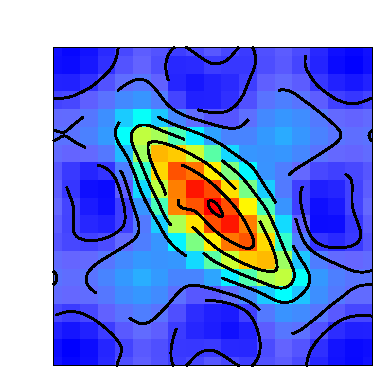
\includegraphics[width={309.00bp},height={223.00bp}]{Q0_E}}%
    \gplfronttext
  \end{picture}%
\endgroup
